% SOURCE_AUTHORITY: sga5_fr_workpass.tex, lines 2610--2744 (LF-normalized unit).
% SOURCE_SHA256: 791F4EFFC5E02832D5D77ED03518C8156D6F07E4C8238B03545DB93D883FBB28
\subsection*{3.6}
Na prática, utiliza-se sobretudo a descrição 3.5 b). Explicitemo-la no nível das classes de cohomologia, supondo, para simplificar a escrita, que $S$ seja o espectro de um corpo separavelmente fechado. Seja
\[
u\in\Hom_S(L_1,L_2)=\Hom(p_1^*L_1,p_2^!L_2).
\]
Para $x\in\H_c^i(X_1,L_1)$, $u_*(x)\in\H^i(X_2,L_2)$ define-se do seguinte modo: considera-se o elemento $p_1^*x\in\H^i(X_2,p_{2!}p_1^*L_1)$ deduzido de $x$ por imagem inversa e aplica-se-lhe $u$, isto é, forma-se o produto
\[
u\cdot p_1^*x\in \H^i(X_2,p_{2!}p_2^!L_2),
\]
e depois aplica-se a flecha
\[
a:\H^i(X_2,p_{2!}p_2^!L_2)\longrightarrow \H^i(X_2,L_2)
\]
definida pela flecha de adjunção $p_{2!}p_2^!\to\Id$; em resumo:
\begin{equation}
u_*(x)=a(u\cdot p_1^*x).
\tag{3.6.1}
\end{equation}
Sejam $c:C\to X$ um morfismo próprio e $u\in\Hom(c_1^*L_1,c_2^!L_2)$. Denotemos por
\[
u_*\in\Hom\bigl(\R\Gamma_c(X_1,L_1),\R\Gamma(X_2,L_2)\bigr)
\]
a imagem de $u$ pela composta de 3.2.3 e 3.3.3. De 3.6.1 deduz-se que, para $x\in\H_c^i(X_1,L_1)$, tem-se
\begin{equation}
u_*(x)=a(u\cdot c_1^*x),
\tag{3.6.2}
\end{equation}
onde $c_1^*x$ é a imagem inversa de $x$ em $\H^i(X_2,c_{2!}c_1^*L_1)$ e
\[
a:\H^i(X_2,c_{2!}c_2^!L_2)\longrightarrow \H^i(X_2,L_2)
\]
é a flecha deduzida da adjunção $c_{2!}c_2^!L_2\to\Id$. Na situação do exemplo 3.2 a), obtém-se assim
\begin{equation}
\operatorname{cl}(c,N)_*(x)=\mathrm{Tr}_{c_2}(c_1^*x),
\tag{3.6.3}
\end{equation}
onde
\[
\mathrm{Tr}_{c_2}:\H^i(X_2,\R c_{2!}A_C)\longrightarrow\H^{i-2N}(X_2,A(-N))
\]
é a flecha induzida pelo morfismo de traço relativo a $c_2$. Esta fórmula concorda, para $N=0$, com (SGA $4^{1/2}$ Ciclo 3.6): $\operatorname{cl}(c)_*$ é o homomorfismo denotado por $\eta_{X_2,X_1}$ em (loc. cit.). Se $X_1$ é suave, de dimensão relativa pura $r_1$, e $c$ é uma imersão fechada, de 3.6.1 e da observação feita no final de 3.2 a) deduz-se que também se tem
\begin{equation}
\operatorname{cl}(c,N)_*(x)=\mathrm{Tr}_{p_2}(\operatorname{cl}(C)\,p_1^*x),
\tag{3.6.4}
\end{equation}
onde $\operatorname{cl}(C)\in \H_C^{2(r_1-N)}(X,A(r_1-N))$ é a classe de cohomologia de $C$ e
\[
\mathrm{Tr}_{p_2}:\H^*(X_2,\R p_{2!}A_X)\longrightarrow \H^{*-2r_1}(X_2,A(-r_1))
\]
é a flecha definida pelo morfismo de traço relativo a $p_2$. Recupera-se a definição habitual do homomorfismo induzido na cohomologia por uma correspondência ([12] 1.3), (SGA $4^{1/2}$ Ciclo 3.2).

\subsection*{3.6.5}
Na situação de 3.2 b), de 3.6.2 deduz-se que, para $u\in\Hom(F^*L_1,L_2)$,
\[
u_*:\H_c^i(X_1,L_1)\longrightarrow \H^i(X_2,L_2)
\]
é a composta do homomorfismo ``imagem inversa''
\[
\H_c^i(X_1,L_1)\longrightarrow \H^i(X_2,F^*L_1)
\]
e do homomorfismo induzido por $u$ (mais geralmente, $f_*u:\R f_{1!}L_1\to \R f_{2*}L_2$ é a composição do homomorfismo canônico
\[
\R f_{1!}L_1\longrightarrow \R f_{2*}F^*L_1
\]
e de $\R f_{2*}u$). Em particular, a correspondência diagonal induz a flecha canônica
\[
\R f_{1!}L_1\longrightarrow \R f_{1*}L_1
\]
(a identidade se $X_1$ é próprio sobre $S$).

\subsection*{3.7}
Voltemos à situação do início de 3.3, supondo dado, além disso, um quadrado comutativo
\begin{equation}
\begin{tikzcd}[column sep=3em,row sep=2em]
X \arrow[d,"f"'] & C \arrow[l,"c"'] \arrow[d,"g"] \\
Y & D \arrow[l,"d"]
\end{tikzcd}
\tag{3.7.1}
\end{equation}
com $c$ próprio. Ponhamos $c_i=p_ic$, $d_i=q_id$, onde $p_i:X\to X_i$, $q_i:Y\to Y_i$ são as projeções. De 3.7.1 deduz-se um diagrama comutativo no qual o quadrado interior é cartesiano:
\begin{equation}
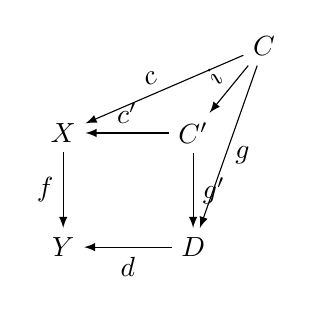
\begin{tikzpicture}[>=latex,baseline=(current bounding box.center),scale=1]
\node (X) at (0,0) {$X$};
\node (Y) at (0,-1.45) {$Y$};
\node (Cp) at (1.65,0) {$C'$};
\node (D) at (1.65,-1.45) {$D$};
\node (C) at (2.55,1.1) {$C$};
\draw[->] (C) -- node[above,sloped,pos=.55] {$c$} (X);
\draw[->] (C) -- node[above,sloped,pos=.50] {$i$} (Cp);
\draw[->] (C) -- node[right,pos=.55] {$g$} (D);
\draw[->] (Cp) -- node[above] {$c'$} (X);
\draw[->] (Cp) -- node[right] {$g'$} (D);
\draw[->] (X) -- node[left] {$f$} (Y);
\draw[->] (D) -- node[below] {$d$} (Y);
\end{tikzpicture}
\tag{3.7.2}
\end{equation}
Para $K\in\ob\Dctf(X)$, tem-se uma flecha canônica
\begin{equation}
f_*c_*c^!K\longrightarrow d_*d^!f_*K,
\tag{3.7.3}
\end{equation}
composta da flecha
\[
f_*c_*c^!K=f_*c'_*(i_*i^!)c'^!K\longrightarrow f_*c'_*c'^!K=d_*g'_*c'^!K
\]
definida pela flecha de adjunção $i_*i^!\to\Id$, e do isomorfismo
\[
d_*g'_*c'^!K\xrightarrow{\sim}d_*d^!f_*K
\]
definido pelo isomorfismo canônico $g'_*c'^!\xrightarrow{\sim}d^!f_*$ (SGA 4 XVIII 3.1.12.3). Tomando $K=\uRHom_S(L_1,L_2)$ e compondo 3.7.3 com o isomorfismo deduzido de 3.3.1, obtém-se uma flecha canônica
\begin{equation}
f_*c_*c^!\uRHom_S(L_1,L_2)
\longrightarrow
 d_*d^!\uRHom_S(f_{1!}L_1,f_{2*}L_2),
\tag{3.7.4}
\end{equation}
que, graças a 3.2.1, pode ser reescrita
\begin{equation}
f_*c_*\uRHom(c_1^*L_1,c_2^!L_2)
\longrightarrow
 d_*\uRHom(d_1^*(f_{1!}L_1),d_2^!(f_{2*}L_2)).
\tag{3.7.5}
\end{equation}
Dela se deduz
\begin{equation}
f_*:\Hom(c_1^*L_1,c_2^!L_2)
\longrightarrow
\Hom(d_1^*(f_{1!}L_1),d_2^!(f_{2*}L_2)).
\tag{3.7.6}
\end{equation}
A flecha 3.7.5 (resp. 3.7.6) generaliza 3.3.1 (resp. 3.3.2), com a qual coincide quando $c$ e $d$ são as identidades. Observe-se também que, para $c$ próprio, 3.2.2 (resp. 3.2.3) não é senão 3.7.5 (resp. 3.7.6) quando $f_1$, $f_2$ e $d$ são as flechas identidade. Quando $Y_1=Y_2=S=D$, abreviaremos $f_*u$ como $u_*$, como antes.

\section{Apareamientos de correspondencias. Fórmula de Lefschetz}
